\documentclass{article}

\usepackage{graphicx}
\usepackage{amsmath}
\graphicspath{ {./images/} }

\usepackage[greek,english]{babel}
\usepackage{alphabeta}



\title{Άσκηση 7}
\author{Χρήστος Αλέξανδρος Τσιγγιρόπουλος}
\date{30 January 2022}


\begin{document}
    \maketitle
    Στην άσκηση αυτή προσεγγίζουμε την συνάρτηση τιμής κλεισίματος με πολυώνυμο δεύτερου 
    τρίτου και τέταρτου βαθμού των κρυπτό νομισμάτων Ethereum και Solana με την μέθοδο των 
    ελαχίστων τετραγώνων. Για τις προσεγγίσεις αυτές χρησιμοποιήθηκαν οι παρακάτω 10 τιμές:
    \begin{equation*}
        ETH\_USD = [1369.04, 1594.76, 1746.62, 1783.80, 1779.79, 1960.16, 1570.20, 1459.97, 1564.71, 1541.91]
    \end{equation*}
    \begin{equation*}
        SOL\_USD = [4.61, 6.43, 7.88, 9.22, 8.86, 11.47, 15.20, 13.20, 14.96, 13.10]
    \end{equation*}
    Για τις μέρες 1,4,8,11,15,19,23,27 Φεβρουαρίου , 29 = 1 Μαρτίου και 32 = 4 Μαρτίου 
    αντίστοιχα (5 Μαρτίου τα γενέθλια μου).
    Αποτέλεσμα του κώδικα είναι η προσέγγιση της τιμής των νομισμάτων αυτών για τις 
     (6 Μαρτίου = 34) και για τις (10 Μαρτίου = 38) για κάθε πολυώνυμο.

    \section{Επεξήγηση Κώδικα}
    Χρησιμοποιούμε την συνάρτηση Elaxista\_Tetragvna(days, prices, 2) που παίρνει τα ορίσματα days, τιμή και τον βαθμό του πολυώνυμου και επιστρέφει έναν πίνακα που 
    για στοιχεία του έχει τους σταθερούς όρους του πολυωνύμου. Η συνάρτηση Elaxista\_Tetragvna\_x(Σταθεροι όροι, day)) παίρνει ως όρισμα τον πίνακα με τους
    σταθερούς όρους του πολυωνύμου που δημιουργήθηκε απο την πιο πάνω συνάρτηση
    και την ημέρα που θέλουμε να προσεγγίσουμε την τιμή της και επιστρέφει την τιμή.
    
    Δλδ δημιουργώ ένα πολυώνυμο p(x) με x την ημέρα και p(x) την τιμή του νομίσματος για την
    ημέρα x.
    
    \section{Αποτέλεσμα Προγράμματος}
 Η τιμή του Ethereum στις 6 Μαρτίου: 1654.74
     Προσέγγιση με πολυώνυμο 2ου βαθμού: 1314.123890
     Προσέγγιση με πολυώνυμο 3ου βαθμού: 1521.763847
     Προσέγγιση με πολυώνυμο 4ου βαθμού: 1681.931758
 Η τιμή του Solana στις 6 Μαρτίου: 13.04
     Προσέγγιση με πολυώνυμο 2ου βαθμού: 14.437751
     Προσέγγιση με πολυώνυμο 3ου βαθμού: 12.799734
     Προσέγγιση με πολυώνυμο 4ου βαθμού: 10.494366

 Η τιμή του Ethereum στις 10 Μαρτίου: 1799.17
     Προσέγγιση με πολυώνυμο 2ου βαθμού: 1069.668345
     Προσέγγιση με πολυώνυμο 3ου βαθμού: 1621.662685
     Προσέγγιση με πολυώνυμο 4ου βαθμού: 2271.121967
 Η τιμή του Solana στις 10 Μαρτίου: 14.23
     Προσέγγιση με πολυώνυμο 2ου βαθμού: 14.569499
     Προσέγγιση με πολυώνυμο 3ου βαθμού: 10.214964
     Προσέγγιση με πολυώνυμο 4ου βαθμού: 0.867009
     
    \section{Σχολιασμός Αποτελεσμάτων}
    Γνωρίζουμε ότι όσο πιο μικρό είναι το $||r||_2$ τόσο καλύτερη είναι η προσέγγιση.
    Το $||r||_2$ γίνεται όλο και πίο μικρό όσο αυξάνεται ο βαθμός του πολυωνύμου.
    Αυτό όμως ισχύει για τις τιμές που εισάχθηκαν, όχι για τις προσεγγίσεις εκτός του ορίου αυτου. 
    Παρατηρούμε ότι για την κοντινότερη τιμή (6 Μαρτίου) η καλύτερη προσέγγιση για το Ethereum είναι αυτή του πολυωνύμου 4ου βαθμού, ενώ για την τιμή στις (10 Μαρτιου) η καλύτερη προσέγγιση είναι αυτή του πολυωνύμου 3ου βαθμού. 
    Για την τιμή του Solana τώρα η καλύτερη προσέγγιση, είναι αυτή του πολυωνύμου του 3ου και 2ου βαθμού αντίστοιχα.
    
    Παρατηρούμε ότι το πολυώνυμο 4ου βαθμού επιρεάζεται αρκετά απο την μεταβολή της τιμής
    των τελευταίων ημερών. 

    Μπορούμε να δούμε τις γραφικές παραστάσεις παρακάτω.

    \section{Γραφικές παραστάσεις}
    Οι γραφικές παραστάσεις υλοποιείται με δύο συναρτήσεις την PlotETH() και την PlotSOL(). Ο κώδικας για αυτές
    είναι υλοποιημένος στο ίδιο αρχείο του προγράμματος απλά έχει μπει σε σχόλια το σημείο που καλούνται.
    ΠΡΟΣΟΧΗ: Δεν μπορουν να χρησιμοποιηθουν ταυτόχρονα στην ίδια εκτέλεση.
    \begin{figure}[b]
    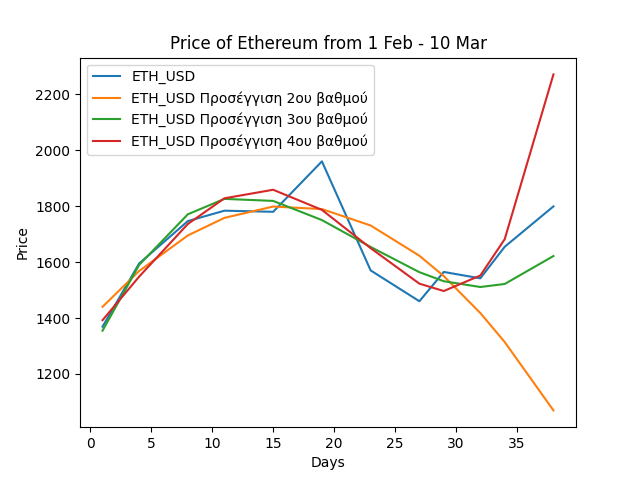
\includegraphics[width=12cm]{ETH_USD.png}
    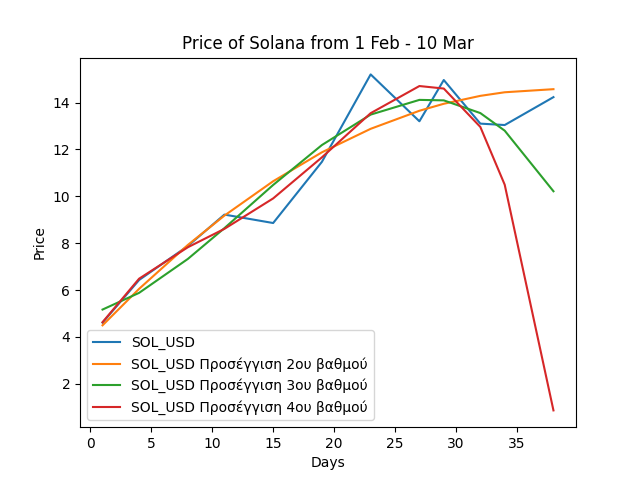
\includegraphics[width=12cm]{SOL_USD.png}
    \end{figure}
    
    
\end{document}